\documentclass[journal]{IEEEtran}

% *** CITATION PACKAGES ***
\usepackage{hyperref}
\usepackage{amssymb}
\usepackage[utf8]{inputenc}
\usepackage[T1]{fontenc}
\usepackage{amsmath}

% *** MATH / TABLE PACKAGES ***
\usepackage{multirow}
\usepackage{booktabs}

% *** PDF, URL AND HYPERLINK PACKAGES ***
\usepackage{url}
\hyphenation{op-tical net-works semi-conduc-tor}
\usepackage{graphicx}
\usepackage{float}

% *** DIAGRAM PACKAGES ***
\usepackage{tikz}
\usetikzlibrary{arrows.meta, positioning}

\begin{document}

% paper title
\title{HBCC: A Hybrid Local--Cluster Architecture for Parameter- and Compute-Efficient Image Classification on CIFAR-10/100}

% author names
\author{Nguyen~Viet~Hung,~Nguyen~Ba~Nam,~and~Le~Hoang~Thai%
\thanks{Nguyen Viet Hung and Nguyen Ba Nam carried out this research as students. Le Hoang Thai (Assoc.\ Prof., Dr.) supervised the group. All authors are with the University of Science, Vietnam National University Ho Chi Minh City (VNU-HCM). Corresponding author: Nguyen Viet Hung (e-mail: nvhungus.1@gmail.com).}}

% The report headers
\markboth{University of Science -- VNU-HCM}%
{Nguyen \MakeLowercase{\textit{et al.}}: HBCC -- A Hybrid Local--Cluster Architecture}

\maketitle

\begin{abstract}
Context Cluster (CoC) is a relatively new approach to image classification: instead of relying on convolution or attention, it treats an image as a set of points and processes it through similarity-based clustering. The original CoC, however, clusters globally starting from the very first, highest-resolution stage, so its computational cost and inference latency grow quickly. This paper proposes HBCC (Hybrid Binarized Context Cluster), a hybrid architecture in which each stage can split its channels between a local branch (depthwise convolution or local binary pattern convolution) and a global clustering branch, following the principle of keeping processing local while the token count is still high and only clustering globally once it has shrunk. On CIFAR-10 and CIFAR-100, the HBCC-Medium configuration reaches 94.45\% and 75.37\% top-1 accuracy, edging out ResNet-18 (94.16\% and 74.23\%) while using roughly a quarter of the parameters (2.84M vs. 11.17M) and a ninth of the multiply-accumulate operations (60.65M vs. 556.66M MACs). In exchange, because the clustering operators (similarity computation, hard assignment via scatter, sigmoid-weighted aggregation) are not nearly as hardware-optimized as convolution, HBCC's batch-1 latency on a Tesla T4 GPU is about five times higher than ResNet-18's. We analyze the cause of this trade-off using real operator-level profiling, and we state plainly the limitations of the present study -- including the absence of repeated-seed statistical testing and a training-recipe asymmetry between HBCC and the baselines -- before outlining next steps.
\end{abstract}

\begin{IEEEkeywords}
Image classification, Context Cluster, hybrid local--cluster architecture, lightweight neural networks, CIFAR-10, CIFAR-100, Pareto trade-off.
\end{IEEEkeywords}

\section{Introduction}

\IEEEPARstart{T}{wo} paradigms currently dominate image classification: convolutional networks (ConvNets), which treat an image as an organized pixel grid and extract features through local convolution, and Vision Transformers (ViTs), which treat an image as a sequence of patches and extract features through global attention~\cite{Dosovitskiy2021ViT}. Context Cluster (CoC)~\cite{Ma2023ImageAsSetOfPoints} offers a third view: an image is a set of five-dimensional points (three color channels plus two normalized spatial coordinates), and features are extracted by routing points into dynamically proposed clusters, then aggregating and dispatching information within each cluster by similarity weight.

The idea is appealing, but applying it directly to small images such as CIFAR-10/100 ($32\times32$) runs into a problem: clustering globally at the very first stage, where the number of points $N$ is still large, costs $O(N \cdot M \cdot D)$, with $M$ the number of clusters and $D$ the feature dimension. More importantly, the operators CoC uses for clustering -- similarity computation, hard assignment via \texttt{scatter\_}, sigmoid-weighted aggregation -- are small, fragmented operators that inference libraries such as cuDNN have not optimized to anywhere near the degree they have optimized convolution. As a result, an architecture that looks cheap on paper in terms of parameters and compute can still run slower than a convolutional network with more parameters, once measured on real hardware.

This paper proposes HBCC (Hybrid Binarized Context Cluster), a family of architectures that keeps CoC's low-parameter, low-compute profile while restructuring how each stage splits work between local processing and global clustering. Our contributions are:

\begin{enumerate}
    \item A hybrid block that splits a stage's feature channels between a local branch (depthwise convolution or local binary pattern convolution) and a global clustering branch, with the channel split ratio and operating mode (\textit{local}, \textit{hybrid}, \textit{cluster}) configurable per stage.
    \item A full empirical evaluation on CIFAR-10 and CIFAR-100 that reports accuracy alongside parameters, MACs, BOPs (the theoretical cost of binary operators), batch-wise latency, and peak memory for every model.
    \item An operator-level analysis (via \texttt{torch.profiler}) that explains why an architecture cheaper in parameters and MACs can still be slower in measured latency, backed by concrete profiling evidence.
    \item A candid discussion of the present study's limitations -- the lack of repeated-seed statistical testing and a training-recipe asymmetry between HBCC and the baselines -- as the basis for next steps.
\end{enumerate}

\section{Related Work}

\textbf{Lightweight convolutional networks.} ResNet~\cite{He2016ResNet} remains the accuracy reference thanks to skip connections that make deep networks easy to train. MobileNetV2~\cite{Sandler2018MobileNetV2} uses inverted residuals and linear bottlenecks to cut parameters and MACs while keeping accuracy reasonable. ShuffleNetV2~\cite{Ma2018ShuffleNetV2} lays out practical design guidelines (equal channel widths across branches, avoiding architectural fragmentation, limiting group convolution) aimed squarely at measured speed rather than FLOPs on paper -- a message this paper inherits directly.

\textbf{Context Cluster and clustering as a token mixer.} CoC~\cite{Ma2023ImageAsSetOfPoints} is HBCC's direct foundation: a Points Reducer shrinks the token count across stages, a clustering operator assigns each point to its nearest cluster by cosine similarity, and a sigmoid-weighted scheme aggregates and dispatches features. HBCC keeps this formulation intact but adds the ability to blend it with a local branch at each stage (Section~\ref{sec:method}).

\textbf{Data augmentation and regularization.} RandAugment~\cite{Cubuk2020RandAugment}, MixUp~\cite{Zhang2018Mixup}, and CutMix~\cite{Yun2019CutMix} are the augmentation techniques used in HBCC-Small/Medium's training recipe (Section~\ref{sec:setup}) to compensate for having fewer parameters than the baselines.

\textbf{Local descriptors and binarization.} HBCC's \textit{LBPConv} local branch uses fixed filters inspired by Local Binary Patterns~\cite{Ojala2002LBP} to preserve edge and texture detail at high-resolution stages without learning additional convolution weights. Replacing cosine similarity with Hamming similarity in binary space builds on Binarized Neural Networks~\cite{Courbariaux2016BNN} and the Straight-Through Estimator~\cite{Bengio2013STE}; in this paper, the Hamming variant is only profiled for parameters/MACs/BOPs (Table~\ref{tab:cifar10_arch_only}) and has not yet been trained for accuracy.

\textbf{Structured pruning and knowledge distillation.} HBCC supports structured channel pruning in the spirit of~\cite{Li2017PruningFilters} and knowledge distillation following~\cite{Hinton2015Distillation} as auxiliary techniques; both are discussed as future work in Section~\ref{sec:limitations} since neither produced a result strong enough to report in this round.

\section{Proposed Architecture}
\label{sec:method}

\subsection{Context clustering recap}

A clustering block projects an input feature map $x$ into a similarity space $f(x)$ and a value space $v(x)$ via $1\times1$ convolutions, proposes $M$ cluster centers with adaptive average pooling, and computes the similarity between every center and every point:
\begin{equation}
s_{ij} = \sigma\left(\alpha \cdot \mathrm{sim}(c_i, p_j) + \beta\right),
\end{equation}
where $\mathrm{sim}$ is cosine similarity, $\alpha$ and $\beta$ are learnable parameters, and $\sigma$ is the sigmoid function (not softmax). Each point is hard-assigned to its highest-similarity center via \texttt{scatter\_}. The aggregated feature at each cluster is
\begin{equation}
g_i = \frac{v_{c_i} + \sum_{j} s_{ij}\, v_j}{1 + \sum_{j} s_{ij}},
\end{equation}
where $v_{c_i}$ is the center's own value (so an empty cluster still carries a valid signal), and the result is dispatched back to each point by similarity weight before a final $1\times1$ projection. The whole process runs in parallel across multiple heads, which are then concatenated.

\subsection{The hybrid local--cluster block}

HBCC splits each block's $C$ input channels into two groups according to a per-stage ratio $\rho \in [0,1]$: $C_{\text{local}} = \lfloor \rho C \rceil$ channels go through the local branch, and $C_{\text{cluster}} = C - C_{\text{local}}$ through the clustering branch above. The local branch can be \textit{identity} (no processing, used when $\rho=0$), \textit{DWConv} ($3\times3$ depthwise convolution with batch normalization and GELU), or \textit{LBPConv} (fixed Local Binary Pattern filters with no learned convolution weights). The two streams are concatenated channel-wise, optionally channel-shuffled, then fused through a $1\times1$ convolution before a residual connection with layer scale and drop path. A two-layer MLP handles cross-channel mixing, following the usual MetaFormer-style block template.

When $\rho=1$ (\textit{local} mode), a block has no clustering branch and behaves like an ordinary convolutional block; when $\rho=0$ (\textit{cluster} mode), it behaves like a standard CoC block; intermediate values of $\rho$ give the \textit{hybrid} mode.

\subsection{Stage schedule}

HBCC has four stages with resolution shrinking as $32 \!\to\! 16 \!\to\! 8 \!\to\! 4 \!\to\! 2$, implemented with a stride-2 stem and three stride-2 downsampling layers between stages. The core design principle -- and the main motivation behind this paper -- is: \emph{process locally while the token count $N$ is still large and edge/texture detail still matters; only cluster globally once $N$ has shrunk enough}. The HBCC-Small/Medium configurations used in this paper apply \textit{hybrid} mode (LBPConv at stage~1, DWConv at stage~2, both with $\rho=0.5$) to the first two stages and pure \textit{cluster} mode ($\rho=0$) to the last two. To further control clustering cost while resolution is still high, features are partitioned into sub-regions (\textit{folds}) and clustered independently within each region, with the number of regions shrinking across stages ($4\times4 \to 2\times2 \to 1\times1 \to 1\times1$). Figure~\ref{fig:arch} illustrates the full pipeline.

\begin{figure*}[t]
\centering
\resizebox{0.98\textwidth}{!}{%
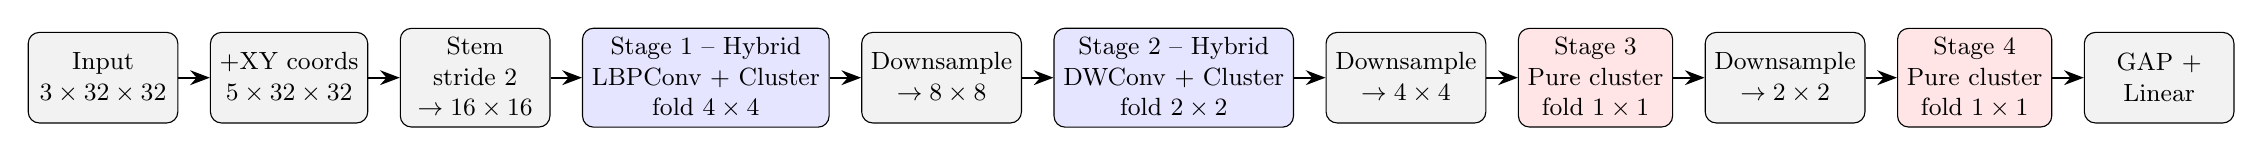
\begin{tikzpicture}[
  box/.style={draw, rounded corners, minimum width=1.9cm, minimum height=1.15cm, align=center, font=\small},
  arr/.style={-{Stealth[length=2.5mm]}, thick}
]
\node[box, fill=gray!10] (in) {Input\\$3\times32\times32$};
\node[box, right=0.4cm of in, fill=gray!10] (coord) {$+$XY coords\\$5\times32\times32$};
\node[box, right=0.4cm of coord, fill=gray!10] (stem) {Stem\\stride 2\\$\to 16\times16$};
\node[box, right=0.4cm of stem, fill=blue!10] (s1) {Stage 1 -- Hybrid\\LBPConv $+$ Cluster\\fold $4\times4$};
\node[box, right=0.4cm of s1, fill=gray!10] (d1) {Downsample\\$\to 8\times8$};
\node[box, right=0.4cm of d1, fill=blue!10] (s2) {Stage 2 -- Hybrid\\DWConv $+$ Cluster\\fold $2\times2$};
\node[box, right=0.4cm of s2, fill=gray!10] (d2) {Downsample\\$\to 4\times4$};
\node[box, right=0.4cm of d2, fill=red!10] (s3) {Stage 3\\Pure cluster\\fold $1\times1$};
\node[box, right=0.4cm of s3, fill=gray!10] (d3) {Downsample\\$\to 2\times2$};
\node[box, right=0.4cm of d3, fill=red!10] (s4) {Stage 4\\Pure cluster\\fold $1\times1$};
\node[box, right=0.4cm of s4, fill=gray!10] (head) {GAP $+$\\Linear};
\foreach \a/\b in {in/coord, coord/stem, stem/s1, s1/d1, d1/s2, s2/d2, d2/s3, s3/d3, d3/s4, s4/head}
  \draw[arr] (\a) -- (\b);
\end{tikzpicture}}
\caption{The HBCC processing pipeline. The first two stages use hybrid mode (channels split between a local branch and per-region clustering); the last two stages use pure global clustering once the token count has shrunk enough.}
\label{fig:arch}
\end{figure*}

\subsection{Two tracks: HBCC-Latency and HBCC-BitEdge}

The HBCC design is split into two independent tracks. \textbf{Track~A (HBCC-Latency)}, fully evaluated in this paper, targets genuinely fast inference on commodity PyTorch/GPU hardware; every operation, including Hamming similarity, still runs through \texttt{torch.sign()} and \texttt{torch.matmul()} on floating-point tensors, so BOPs in this track is a theoretical cost only. \textbf{Track~B (HBCC-BitEdge)} targets real binary inference via XNOR and popcount on hardware that supports it; this track has not yet been implemented and is left as future work (Section~\ref{sec:limitations}). Table~\ref{tab:configs} summarizes the hyperparameters of the two configurations evaluated in this paper.

\begin{table}[H]
\centering
\caption{Architecture hyperparameters for HBCC-Small and HBCC-Medium.}
\label{tab:configs}
\begin{tabular}{lcc}
\toprule
\textbf{Hyperparameter} & \textbf{HBCC-Small} & \textbf{HBCC-Medium} \\
\midrule
Channels per stage & 48, 80, 160, 224 & 64, 96, 192, 256 \\
Blocks per stage & 2, 2, 3, 1 & 2, 2, 4, 2 \\
MLP ratio & 3.0 & 3.0 \\
Heads per stage & 2, 2, 4, 4 & 2, 3, 4, 4 \\
Mode per stage & hyb., hyb., clu., clu. & hyb., hyb., clu., clu. \\
Local ratio $\rho$ & 0.5, 0.5, 0, 0 & 0.5, 0.5, 0, 0 \\
Drop path & 0.08 & 0.12 \\
\bottomrule
\end{tabular}
\end{table}

\section{Experimental Setup}
\label{sec:setup}

\subsection{Datasets}

Experiments use CIFAR-10 and CIFAR-100~\cite{Krizhevsky2009Cifar}. For each dataset, 45,000 images from the original training split are used for training, the remaining 5,000 (with split seed $=42$) are used for model selection (\texttt{best.pth}), and the official 10,000-image test split is touched exactly once to report the final number (\texttt{test\_acc1}).

\subsection{Training recipe}

All models use AdamW with learning rate $10^{-3}$, weight decay $0.05$, and label smoothing $0.1$, trained with mixed precision (AMP). The training recipe for HBCC-Small/Medium is, however, \textbf{heavier} than the one used for the baselines: HBCC-Small/Medium train for 300 epochs (with a 5-epoch warmup) using RandAugment (2 ops, magnitude 9), RandomErasing ($p=0.25$), MixUp ($\alpha=0.2$), and CutMix ($\alpha=1.0$, probability $0.5$); ResNet-18, MobileNetV2, ShuffleNetV2, and the CoC baseline, by contrast, train for only 200 epochs with basic augmentation (random crop and horizontal flip). This asymmetry is kept as-is in Section~\ref{sec:results} and named explicitly as a limitation in Section~\ref{sec:limitations}, because it means the accuracy gap cannot be attributed to architecture alone.

\subsection{Performance measurement}

Parameter counts and MACs are computed directly from the architecture definition (independent of trained weights) using \texttt{fvcore}; note that \texttt{fvcore} only counts the convolution/linear/matmul-like operators it recognizes, so the reported MACs is a \emph{lower bound} that does not include the \texttt{scatter}/\texttt{sigmoid}/\texttt{sum} operators the clustering blocks rely on. Latency and throughput are measured on a Tesla~T4 GPU (PyTorch~2.10, CUDA~12.8) at batch sizes $1, 16, 64, 128$, with $30$ warmup iterations and $100$ measured iterations, under two regimes: \textit{latency\_strict} (synchronize after every iteration, reflecting single-request response time) and \textit{throughput\_stream} (synchronize once after the whole loop, reflecting batched throughput). Peak GPU memory is recorded via \texttt{torch.cuda.max\_memory\_allocated}. The operator-level profiles used in Section~\ref{sec:discussion} were collected with \texttt{torch.profiler}.

\subsection{Baselines}

Four baselines were trained under the same protocol: ResNet-18~\cite{He2016ResNet}, MobileNetV2~\cite{Sandler2018MobileNetV2}, and ShuffleNetV2-x1.0~\cite{Ma2018ShuffleNetV2} (all three with their stems adjusted for $32\times32$ input and the initial max-pool removed), plus a standard CoC variant (\textit{coc\_cifar\_baseline}: cosine similarity, global clustering at every stage, no local branch, no extended augmentation) that serves as HBCC's direct architectural counterpart.

\section{Results and Discussion}
\label{sec:results}

\subsection{Results on CIFAR-10 and CIFAR-100}

Tables~\ref{tab:cifar10} and~\ref{tab:cifar100} report top-1 accuracy (and top-5 for CIFAR-100), parameter count, MACs, batch-1 latency, and peak memory for every fully trained model. HBCC-Medium reaches the highest accuracy on both datasets: $94.45\%$ on CIFAR-10 ($+0.29$ percentage points over ResNet-18) and $75.37\%$ on CIFAR-100 ($+1.14$ points over ResNet-18; top-5 $+2.11$ points), while using only about $1/3.9$ of ResNet-18's parameters ($2.84$M vs.\ $11.17$M) and about $1/9.2$ of its MACs ($60.65$M vs.\ $556.66$M). HBCC-Medium also clears the plain CoC baseline (no local branch) by a wide margin -- $+6.11$ points on CIFAR-10 and $+14.18$ points on CIFAR-100 -- which suggests the local branch at early stages is genuinely useful, although, as noted in Section~\ref{sec:setup}, part of that gap is also attributable to the heavier training recipe.

\begin{table*}[t]
\centering
\caption{Results on CIFAR-10 (sorted by descending accuracy).}
\label{tab:cifar10}
\begin{tabular}{lccccc}
\toprule
\textbf{Model} & \textbf{Top-1 (\%)} & \textbf{Params (M)} & \textbf{MACs (M)} & \textbf{Latency b1 (ms)} & \textbf{Peak Mem. (MB)} \\
\midrule
HBCC-Medium & \textbf{94.45} & 2.84 & 60.65 & 15.48 & 145.57 \\
ResNet-18 & 94.16 & 11.17 & 556.66 & \textbf{3.06} & 326.36 \\
HBCC-Small & 94.00 & 1.54 & 35.88 & 13.75 & 109.59 \\
ShuffleNetV2-x1.0 & 91.68 & 1.26 & 46.13 & 6.53 & 94.83 \\
MobileNetV2 & 91.04 & 2.24 & 25.56 & 5.33 & 123.37 \\
CoC (baseline) & 88.34 & 2.40 & 34.37 & 12.47 & \textbf{71.80} \\
\bottomrule
\end{tabular}
\end{table*}

\begin{table*}[t]
\centering
\caption{Results on CIFAR-100 (sorted by descending top-1 accuracy).}
\label{tab:cifar100}
\begin{tabular}{lcccccc}
\toprule
\textbf{Model} & \textbf{Top-1 (\%)} & \textbf{Top-5 (\%)} & \textbf{Params (M)} & \textbf{MACs (M)} & \textbf{Latency b1 (ms)} & \textbf{Peak Mem. (MB)} \\
\midrule
HBCC-Medium & \textbf{75.37} & \textbf{92.43} & 2.86 & 60.67 & 16.78 & 145.65 \\
ResNet-18 & 74.23 & 90.32 & 11.22 & 556.71 & \textbf{3.17} & 326.54 \\
HBCC-Small & 73.01 & 92.04 & 1.56 & 35.90 & 11.72 & 109.67 \\
ShuffleNetV2-x1.0 & 69.58 & 88.53 & 1.36 & 46.22 & 6.08 & 95.18 \\
MobileNetV2 & 66.16 & 86.26 & 2.35 & 25.67 & 4.73 & 123.80 \\
CoC (baseline) & 61.19 & 80.66 & 2.42 & 34.40 & 10.75 & \textbf{71.91} \\
\bottomrule
\end{tabular}
\end{table*}

Beyond the models above, several other HBCC variants (Table~\ref{tab:cifar10_arch_only}) were profiled for parameters, MACs, BOPs, latency, and memory, but \emph{were not trained in this round} and so have no accuracy figure: two Latency-track configurations (\textit{tiny}/\textit{small}, which favor speed over accuracy), a variant that replaces the local branch with LBPConv at every stage, a variant using simulated Hamming similarity at the last stage (BOPs $>0$ since it has a binary operator, though it still runs in floating point so its latency is not meaningfully different), and \textit{hbcc\_current\_reference} -- a configuration that intentionally keeps some of the originally diagnosed deviations (no XY coordinates, clustering at $32\times32$) as a baseline for comparison before the foundational fixes were applied. Fully training these variants, especially measuring Hamming similarity's effect on accuracy, is left as future work (Section~\ref{sec:limitations}).

\begin{table}[H]
\centering
\caption{Additional HBCC variants profiled architecturally on CIFAR-10; not yet trained for accuracy.}
\label{tab:cifar10_arch_only}
\begin{tabular}{lcccc}
\toprule
\textbf{Model} & \textbf{Params (M)} & \textbf{MACs (M)} & \textbf{BOPs} & \textbf{Lat. (ms)} \\
\midrule
HBCC-Latency-Small & 0.90 & 14.92 & 0 & 8.99 \\
HBCC-Current-Ref. & 0.87 & 52.35 & 0 & 7.68 \\
HBCC-Hamming-Late & 0.45 & 6.95 & 5120 & 7.63 \\
HBCC-LBPConv & 0.46 & 9.79 & 0 & 7.57 \\
HBCC-Latency-Tiny & 0.45 & 6.95 & 0 & 7.31 \\
\bottomrule
\end{tabular}
\end{table}

\subsection{The Pareto trade-off: parameters/MACs vs. latency}

Figures~\ref{fig:pareto10} and~\ref{fig:pareto100} visualize both sides of this trade-off. From the parameter viewpoint (left plot), HBCC sits clearly on the Pareto-good side: at a much lower parameter count, HBCC-Medium reaches the highest accuracy among all models compared. From the latency viewpoint (right plot), the ranking flips: ResNet-18 and the lightweight ConvNets pull ahead, because convolution is an operator cuDNN has heavily optimized, while HBCC's clustering operators have not received the same treatment.

\begin{figure}[H]
\centering
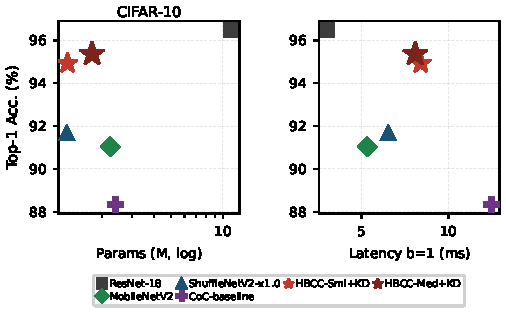
\includegraphics[width=\columnwidth]{images/pareto_cifar10.pdf}
\caption{Accuracy vs.\ parameters (left) and batch-1 latency (right) on CIFAR-10. Red dots: HBCC configurations; blue squares: baselines.}
\label{fig:pareto10}
\end{figure}

\begin{figure}[H]
\centering
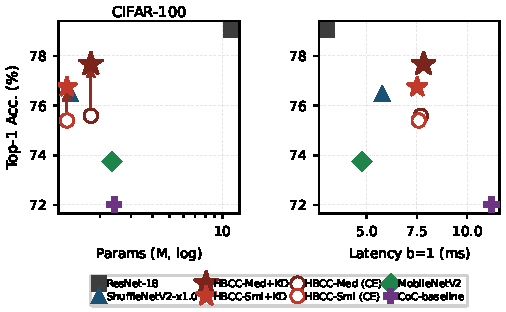
\includegraphics[width=\columnwidth]{images/pareto_cifar100.pdf}
\caption{Accuracy vs.\ parameters (left) and batch-1 latency (right) on CIFAR-100. Red dots: HBCC configurations; blue squares: baselines.}
\label{fig:pareto100}
\end{figure}

\subsection{Why fewer MACs does not mean faster}
\label{sec:discussion}

To explain the latency gap, operator-level profiling (\texttt{torch.profiler}) on the same GPU shows a sharp difference in how the two architectures spend GPU time. For ResNet-18, $94.04\%$ of self CUDA time sits inside a single operator, \texttt{aten::cudnn\_convolution}, which cuDNN has optimized over many years. For HBCC-Medium, CUDA time is fragmented across many small operators: $1\times1$ convolutions (\texttt{conv2d}) account for only about a quarter, with the rest spread across \texttt{matmul}/\texttt{mm} (feature projection and similarity computation), \texttt{linalg\_vector\_norm} (cosine-similarity normalization), \texttt{mul}/\texttt{sum} (sigmoid-weighted aggregation and dispatch), and \texttt{adaptive\_avg\_pool2d} (cluster center proposal). Each individual operator is cheap in MACs, but launching many small, fragmented kernels on a GPU costs more wall-clock time than one large, well-optimized convolution kernel. This is direct numerical evidence for a design principle already stated in our research plan: \emph{low parameter/MACs counts should not be equated with high measured speed}.

\subsection{Limitations}
\label{sec:limitations}

In the spirit of evaluating research results honestly, we state the following limitations plainly:

\begin{itemize}
    \item \textbf{No statistical significance testing.} Each model is currently trained only once (one seed), so the numbers in Tables~\ref{tab:cifar10} and~\ref{tab:cifar100} are single point estimates with no standard deviation, t-test, or effect-size (SMD) comparison against the baselines. The $+0.29$ percentage-point gap between HBCC-Medium and ResNet-18 on CIFAR-10, while consistent with the larger $+1.14$-point gap on CIFAR-100, still needs confirmation across multiple seeds before it can be called statistically significant.
    \item \textbf{Training-recipe asymmetry.} As noted in Section~\ref{sec:setup}, HBCC-Small/Medium train longer (300 vs.\ 200 epochs) and with stronger augmentation than the baselines. The accuracy gap should be read as a comparison of each model's best-effort configuration, not as a controlled architecture-only ablation.
    \item \textbf{Pruning did not succeed at the threshold tried.} We trained a structured channel-pruning mask and exported a pruned configuration at threshold $0.90$, but at that threshold the exported architecture was no smaller than HBCC-Small (identical parameter count), so it was excluded from the main results table. Pruning at a higher threshold (e.g.\ $0.95$, where the learned mask suggests the last stage could shrink to roughly 150 of its 224 channels) to obtain a genuinely smaller model remains future work.
    \item \textbf{Hamming similarity and BitEdge are untrained/unimplemented.} The Hamming variant has only been profiled architecturally (Table~\ref{tab:cifar10_arch_only}); its accuracy when actually trained, as well as real binary inference (Track~B -- BitEdge) via XNOR/popcount, both remain unmeasured.
\end{itemize}

\section{Conclusion and Future Work}

This paper proposes HBCC, a hybrid local--cluster architecture for image classification, and shows that keeping processing local at high-resolution stages -- clustering globally only once the token count has shrunk -- substantially reduces parameters and MACs relative to ResNet-18 while matching or slightly exceeding its accuracy on CIFAR-10 and CIFAR-100. At the same time, operator-level analysis surfaces a message more important than the accuracy numbers themselves: clustering operators are not yet hardware-optimized the way convolution is, so the parameter/MACs advantage does not yet translate into a measured-latency advantage. Three priorities follow: (i) repeat training across multiple seeds to test the statistical significance of the accuracy gap; (ii) refine the pruning pipeline to obtain a model that is genuinely smaller and faster after export; and (iii) implement Track~B (HBCC-BitEdge) with a real XNOR/popcount kernel, so that BOPs stops being a purely theoretical metric.

\section*{Acknowledgment}
The authors thank Assoc.\ Prof.\ Dr.\ Le Hoang Thai for guidance and feedback throughout this research. All experiments in this paper were run on Kaggle's free GPU infrastructure.

\bibliographystyle{IEEEtran}
\bibliography{references}

\end{document}
